\subsubsection{Actors}
There are two actors of this system is the administrator, a bartender or a bar owner in charge of the music, and the guest, wanting to request and affect the music. From this

\begin{table}[h]
\centering
\begin{tabular}{lcc}
\hline
                   & \multicolumn{1}{l}{\textbf{Actor}} & \multicolumn{1}{l}{} \\
\textbf{Use case}  & Administrator                      & Customer             \\ \hline
play music         & \checkmark                         &                      \\
stop music         & \checkmark                         &                      \\
next track         & \checkmark                         &                      \\
add restriction    & \checkmark                         &                      \\
remove restriction & \checkmark                         &                      \\
check out          &                                    & \checkmark           \\
check in at venue  &                                    & \checkmark           \\
vote               &                                    & \checkmark           \\
cancel vote        &                                    & \checkmark           \\ \hline
\end{tabular}
\caption{Actor table for the project}
\end{table}

\actortable{Administrator}{
    \textbf{Purpose:} A person that protects the interests of the venue and is responsible for the music. He or she wants to be able to have control over the system, what kind and in which order music is being enqueued and what is currently playing.

    \textbf{Characteristics:} Has a preference or a theme of music that the individual is following, set by the organisation or the individual itself. Work at the venue and has a reasonable high technical level or the ability and motivation to be thought in the use of the system.

    \textbf{Possible usage:} Administrator A is very open minded for all requests and votes from users and only sets the bare minimum restrictions to keep the theme of the venue.
		
		Administrator B completely controls the playlist by adding, removing and rearranging to completely fit the venues preferences and what is played. He is very restrictive and only accepts requests and votes that he agrees with.
		
		Add and remove restrictions, play, pause and stop music, play next track and add, remove and rearrange tracks on the playlist.\\\\
		Diagram of possible usage, see \cref{fig:UsageAdmin}
}

\begin{figure}[H]
  \centering
  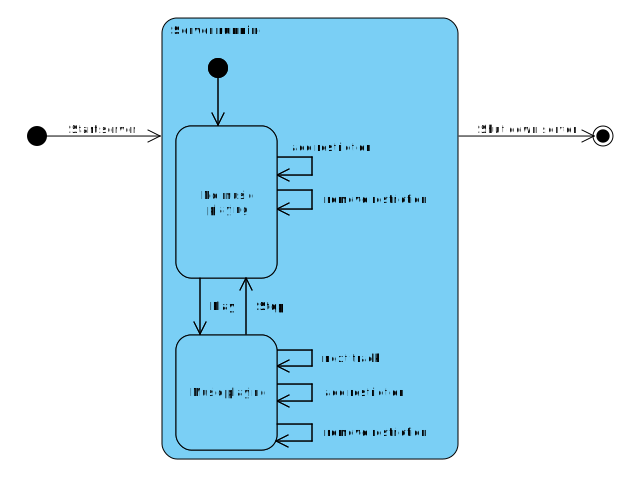
\includegraphics[width=0.7\linewidth]{Images/UsageAdmin.pdf}
  \caption{Usage for a administrator}
  \label{fig:UsageAdmin}
\end{figure}

\actortable{Guest}{
    \textbf{Purpose:} Wants to influence the playlist and listen to preferred tracks at the venue, the individual is visiting.

    \textbf{Characteristics:} Has a music preference possibly different from the administrator and/or the theme, at the specific venue. Varying technical level but with the ability to use his or her specific smartphone and knowledge of native applications.

    \textbf{Possible usage:} Guest A only requests tracks to the playlist but rarely votes on other users tracks.
		
		Guest B only votes on tracks and does not use the feature of requesting tracks.
		
		A user has the ability to check in and out of venue, vote and revote for track and cancel their vote.\\\\
		Diagram of possible usage, see \cref{fig:UsageUser}
}
\begin{figure}[H]
  \centering
  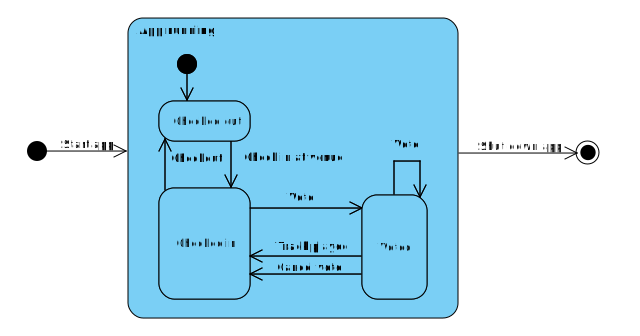
\includegraphics[width=0.7\linewidth]{Images/UsageUser.pdf}
  \caption{Usage for a guest}
  \label{fig:UsageUser}
\end{figure}
